% Author: Jan Schaumann <jschauma@netmeister.org>
% $Id: slides.tex,v 1.5 2006/04/10 14:22:04 jschauma Exp $
\special{! TeXDict begin /landplus90{true}store end }

\documentclass[xga]{xdvislides}
\usepackage[landscape]{geometry}
\usepackage{graphics}
\usepackage{graphicx}
\usepackage{colordvi}
\usepackage{multirow}

\begin{document}
\setfontphv

%%% Headers and footers
\lhead{\slidetitle}                               % default:\lhead{\slidetitle}
\chead{CS615 - Aspects of System Administration}% default:\chead{\relax}
\rhead{Slide \thepage}                       % default:\rhead{\sectiontitle}
\lfoot{\Gray{Popular Services -- HTTP, SNMP}}% default:\lfoot{\slideauthor}
\cfoot{\relax}                               % default:\cfoot{\relax}
\rfoot{\Gray{\today}}

\newcommand{\smallish}{\fontsize{16}{16}\selectfont}

\vspace*{\fill}
\begin{center}
	\Hugesize
		CS615 - Aspects of System Administration\\ [1em]
		Popular Services -- SNMP, HTTP\\ [1em]
	\hspace*{5mm}\blueline\\ [1em]
	\Normalsize
		Department of Computer Science\\
		Stevens Institute of Technology\\
		Jan Schaumann\\
		\verb+jschauma@stevens.edu+\\
		\verb+http://www.cs.stevens.edu/~jschauma/615/+
\end{center}
\vspace*{\fill}

\subsection{SNMP}
\vspace{.5in}
\begin{center}
	\Huge
	A complete network management system to monitor network-attached devices.
\end{center}
\Normalsize

\subsection{SNMP}
Base concepts:
\begin{itemize}
	\item managed devices run an {\em snmp agent} or d\ae mon
	\item information about the device is exposed in {\em management information bases}
	\item parts of a system are made available in {\em read-only} mode
	\item parts of a system may be made available in {\em write} mode
	\item certain conditions may trigger actions or {\em traps}
	\item normally uses UDP 161 for the {\em agent} and 162 for the {\em manager}
\end{itemize}

\subsection{SNMP}
Management Information Bases (MIBs):
\begin{itemize}
	\item hierarchical namespace
	\item contains {\em Object Identifiers} (OIDs)
	\item written in {\em Abstract Syntax Notation One} (ASN.1)
	\item often vendor defined
\end{itemize}

\subsection{SNMP Versions}
SNMPv1:
\begin{itemize}
	\item de-facto standard
	\item poor security (``community strings'' act as passwords)
\end{itemize}
\vspace{.2in}
SNMPv2:
\begin{itemize}
	\item improvements in the area of performance (\verb+GETBULK+ instead of \verb+GETNEXT+) and security
	\item comes in the flavors {\em SNMPv2c}, {\em SNMPv1.5} and {\em SNMPv2u}
\end{itemize}
\vspace{.2in}
SNMPv3:
\begin{itemize}
	\item official standard
	\item adds authentication, privacy and access control
\end{itemize}

\subsection{SNMP: An example}
\smallish
\begin{verbatim}
$ snmpwalk -c public -v 1 colt45.cs.stevens.edu
SNMPv2-MIB::sysDescr.0 = STRING: HP ETHERNET MULTI-ENVIRONMENT,ROM
R.22.01,JETDIRECT,JD95,EEPROM R.24.06,CIDATE 10/17/2002
SNMPv2-MIB::sysObjectID.0 = OID: SNMPv2-SMI::enterprises.11.2.3.9.1
DISMAN-EVENT-MIB::sysUpTimeInstance = Timeticks: (276616180) 32 days, 0:22:41.80
[...]
RFC1213-MIB::ipRouteNextHop.0.0.0.0 = IpAddress: 155.246.81.1
[...]
HOST-RESOURCES-MIB::hrMemorySize.0 = INTEGER: 65536 KBytes
[...]
SNMPv2-SMI::mib-2.43.16.5.1.2.1.1 = STRING: "Powersave on"
[...]
\end{verbatim}


\subsection{SNMP: An example}
\smallish
\begin{verbatim}
$ snmpwalk -c public -v 1 gw.cc.stevens-tech.edu
SNMPv2-MIB::sysDescr.0 = STRING: Cisco IOS Software, s72033_rp Software
(s72033_rp-ADVIPSERVICESK9_WAN-M), Version 12.2(33)SXH, RELEASE SOFTWARE (fc5)
DISMAN-EVENT-MIB::sysUpTimeInstance = Timeticks: (3112108803) 360 days, 4:44:48.03
SNMPv2-MIB::sysContact.0 = STRING: chose@stevens.edu x5457
SNMPv2-MIB::sysName.0 = STRING: gw.cc.stevens-tech.edu
SNMPv2-MIB::sysLocation.0 = STRING: campus:sl:0:machineroom
SNMPv2-MIB::sysORLastChange.0 = Timeticks: (0) 0:00:00.00
[...]
IF-MIB::ifPhysAddress.1 = STRING: 0:17:95:68:d2:dc
IF-MIB::ifPhysAddress.2 = STRING: 0:18:74:1c:e3:80
[...]
IF-MIB::ifAdminStatus.1 = INTEGER: up(1)
IF-MIB::ifAdminStatus.2 = INTEGER: down(2)
[...]
IF-MIB::ifInOctets.1 = Counter32: 147341347
IF-MIB::ifInOctets.2 = Counter32: 487894092
[...]
IF-MIB::ifOutOctets.1 = Counter32: 956876160
IF-MIB::ifOutOctets.2 = Counter32: 1532452749
[...]
RFC1213-MIB::ipRouteDest.66.193.255.0 = IpAddress: 66.193.255.0
RFC1213-MIB::ipRouteDest.66.194.0.0 = IpAddress: 66.194.0.0
[...]
\end{verbatim}
\Normalsize

\subsection{SNMP: An example}
\smallish
\begin{verbatim}
$ snmpwalk -Os -c public -v 1 localhost
sysDescr.0 = STRING: Linux eva 2.6.32-33-generic #72-Ubuntu SMP Fri Jul 29 21:07:13 UTC 2011 x86_64
sysObjectID.0 = OID: netSnmpAgentOIDs.10
sysUpTimeInstance = Timeticks: (90638910) 10 days, 11:46:29.10
sysContact.0 = STRING: Root <root@localhost> (configure /etc/snmp/snmpd.local.conf)
sysName.0 = STRING: eva
sysLocation.0 = STRING: Unknown (configure /etc/snmp/snmpd.local.conf)
[...]
\end{verbatim}

\subsection{Monitoring/graphing}
SNMP based:
\begin{itemize}
	\item Cacti: \verb+http://www.cacti.net/+
	\item MRTG: \verb+http://oss.oetiker.ch/mrtg/+
	\item Observium: \verb+http://demo.observium.org/+
	\item ...
\end{itemize}
\vspace{.2in}
Other / complementary:
\begin{itemize}
	\item Ganglia: \verb+http://monitor.millennium.berkeley.edu/+
	\item Munin: \verb+http://munin.ping.uio.no/+
	\item Nagios: \verb+http://nagioscore.demos.nagios.com/+
	\item Graphite: \verb+http://graphite.wikidot.com/+
\end{itemize}
\vspace{.5in}
%More on monitoring and performance in a future lecture (if time permits).

\newpage
\vspace*{\fill}
\begin{center}
	\Hugesize
		Hypertext Transfer Protocol\\ [1em]
	\hspace*{5mm}
	\blueline\\
	\hspace*{5mm}\\
		Today's Universal Internet Pipe
\end{center}
\vspace*{\fill}



\subsection{HTTP: Hypertext}
\vspace{.5in}
\begin{center}
	\Huge
	W W W
\end{center}
\Normalsize

\subsection{HTTP: Hypertext}
\vspace{.5in}
\begin{center}
	\Huge
	W W W
	\\
\vspace{.5in}
	{\em ``The World Wide Web is the only thing I know of whose shortened form
	takes three times longer to say than what it's short for.'' -- Douglas Adams}
\end{center}
\Normalsize


\subsection{HTTP: Hypertext}
\begin{center}
	\includegraphics[scale=0.9]{pics/http-proposal-detail.eps} \\
	\vspace{.5in}
	\verb+http://is.gd/JnZaN6+
\end{center}

\subsection{HTTP}
\vspace{.5in}
\begin{center}
	\Huge
	Hypertext Transfer Protocol
	\\
	\vspace{.5in}
	RFC2616
\end{center}
\Normalsize

\subsection{HTTP}
\vspace{.5in}
\begin{center}
	\Huge
	HTTP is a request/response protocol.
\end{center}
\Normalsize

\subsection{The Hypertext Transfer Protocol}
HTTP is a request/response protocol:
\begin{enumerate}
	\item client sends a request to the server
	\item server responds
\end{enumerate}

\subsection{The Hypertext Transfer Protocol}
HTTP is a request/response protocol:
\begin{enumerate}
	\item client sends a request to the server
		\begin{itemize}
			\item request method
			\item URI
			\item protocol version
			\item request modifiers
			\item client information
		\end{itemize}
	\item server responds
\end{enumerate}

\subsection{HTTP: A client request}
\vspace*{.5in}
\\
\Hugesize
\begin{center}
\begin{verbatim}
$ telnet www.google.com 80
Trying 173.194.75.147...
Connected to www.google.com.
Escape character is '^]'.
GET / HTTP/1.0
\end{verbatim}
\end{center}
\Normalsize
\vspace*{\fill}


\subsection{The Hypertext Transfer Protocol}
HTTP is a request/response protocol:
\begin{enumerate}
	\item client sends a request to the server
		\begin{itemize}
			\item request method
			\item URI
			\item protocol version
			\item request modifiers
			\item client information
		\end{itemize}
	\item server responds
		\begin{itemize}
			\item status line (including success or error code)
			\item server information
			\item entity metainformation
			\item content
		\end{itemize}
\end{enumerate}

\subsection{HTTP: a server response}
%\smallish
\begin{verbatim}
HTTP/1.0 200 OK
Date: Sun, 31 Mar 2013 01:54:40 GMT
Set-Cookie: PREF=ID=c5eb56d629b347cc:FF=0:TM=1364694880:LM=1364694880:
S=sIdRFdxV9YvtQOlG; expires=Tue, 31-Mar-2015 01:54:40 GMT; path=/;
domain=.google.com
Set-Cookie: NID=67=hvBnOob2NoZW4haTJVfajbcyn_jips50lKRe-8nawzdCZ6AukNR
_s8CNHD6ZA-Z2721nA3TpLrNXt-2zyIui23j4kdsdF8Gg--PmGsMOJ3Jv5frEzQG1elHJv92HL-w2;
expires=Mon, 30-Sep-2013 01:54:40 GMT; path=/; domain=.google.com; HttpOnly
Server: gws

<!doctype html><html itemscope="itemscope" itemtype="http://schema.org/WebPage">
<head><meta content="Search the...

\end{verbatim}
%\Normalsize

\subsection{The Hypertext Transfer Protocol}
Server status codes:
\begin{itemize}
	\item {\bf 1xx} -- Informational; Request received, continuing process
	\item {\bf 2xx} -- Success; The action was successfully received,
        understood, and accepted
	\item {\bf 3xx} -- Redirection; Further action must be taken in order to
        complete the request
	\item {\bf 4xx} -- Client Error; The request contains bad syntax or
		cannot be fulfilled
	\item {\bf 5xx} -- Server Error; The server failed to fulfill an
		apparently valid request
\end{itemize}

\subsection{HTTP: A client request}
\smallish
\begin{verbatim}
$ telnet www.cs.stevens.edu 80
Trying 155.246.89.84...
Escape character is '^]'.
GET / HTTP/1.0

HTTP/1.1 302 Found
Date: Mon, 01 Apr 2013 20:58:35 GMT
Server: Apache/2.2.16 (Debian)
Location: http://www.stevens.edu/compsci
Vary: Accept-Encoding
Content-Length: 312
Content-Type: text/html; charset=iso-8859-1

<!DOCTYPE HTML PUBLIC "-//IETF//DTD HTML 2.0//EN">
<html><head>
<title>302 Found</title>
</head><body>
<h1>Found</h1>
<p>The document has moved <a
href="http://www.stevens.edu/compsci">here</a>.</p>
<hr>
<address>Apache/2.2.16 (Debian) Server at tarantula.srcit.stevens-tech.edu
Port 80</address>
</body></html>
\end{verbatim}
\Normalsize

\subsection{HTTP: A client request}
\smallish
\begin{verbatim}
$ telnet www.stevens.edu 80
Trying 155.246.21.84...
Connected to rweb.cc.stevens.edu.
Escape character is '^]'.
GET /compsci HTTP/1.0

HTTP/1.1 301 Moved Permanently
Date: Mon, 01 Apr 2013 21:06:45 GMT
Location: http://www.stevens.edu/compsci/
Vary: Accept-Encoding
Content-Length: 326
Content-Type: text/html; charset=iso-8859-1

<!DOCTYPE HTML PUBLIC "-//IETF//DTD HTML 2.0//EN">
<html><head>
<title>301 Moved Permanently</title>
</head><body>
<h1>Moved Permanently</h1>
<p>The document has moved <a
href="http://web1v6.stevens.edu/compsci/">here</a>.</p>
</p>
<hr>
<address>Apache/2.2.16 (Debian) Server at web1v6.stevens.edu Port 80</address>
</body></html>
\end{verbatim}
\Normalsize

\subsection{HTTP: A client request}
\smallish
\begin{verbatim}
$ telnet www.stevens.edu 80
Trying 155.246.21.84...
Connected to rweb.cc.stevens.edu.
Escape character is '^]'.
GET /compsci/ HTTP/1.0

HTTP/1.1 302 Moved Temporarily
Date: Mon, 01 Apr 2013 21:08:58 GMT
Server: Apache/2.2.16 (Debian)
X-Powered-By: PHP/5.3.3-7+squeeze8
location: home.php
Vary: Accept-Encoding
Content-Length: 0
Content-Type: text/html
Via: 1.0 www.stevens.edu
Connection: close

Connection closed by foreign host.
\end{verbatim}

\subsection{HTTP: A client request}
\smallish
\begin{verbatim}
$ telnet www.stevens.edu 80
Trying 155.246.21.84...
Connected to rweb.cc.stevens.edu.
Escape character is '^]'.
GET /compsci/home.php HTTP/1.0

HTTP/1.1 200 OK
Date: Mon, 01 Apr 2013 21:09:42 GMT
Server: Apache/2.2.16 (Debian)
X-Powered-By: PHP/5.3.3-7+squeeze8
Vary: Accept-Encoding
Content-Type: text/html
Via: 1.0 www.stevens.edu
Connection: close

<!DOCTYPE html
	PUBLIC "-//W3C//DTD HTML 4.0 Transitional//EN">
<html>
<head>
\end{verbatim}

\subsection{Firebug}
\begin{center}
	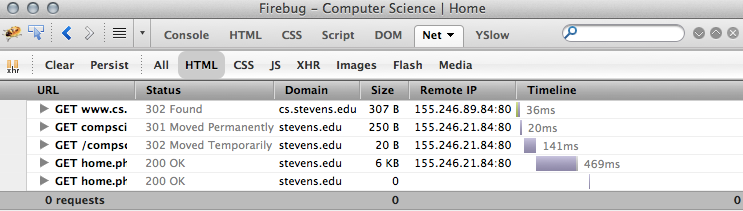
\includegraphics[scale=0.8]{pics/firebug.eps}
\end{center}



\subsection{HTTP - more than just text}
HTTP is a {\em Transfer Protocol} -- serving {\em data}, not any specific
text format.

\begin{itemize}
	\item {\tt Accept-Encoding} client header can specify different formats
		such as {\em gzip}, {\em Shared Dictionary Compression over HTTP (SDCH)} etc.
	\item corresponding server headers: {\tt Content-Type} and
		{\tt Content-Encoding}
\end{itemize}
\begin{center}
	
\includegraphics[scale=2.0]{pics/datatransfer.eps}
\end{center}

\subsection{HTTP - more than just static data}
HTTP is a {\em Transfer Protocol} -- what is transferred need not be
static; resources may generate different data to return based on many
variables.

\begin{itemize}
	\item CGI -- resource is {\em executed}, needs to generate
		appropriate response headers
	\item server-side scripting (ASP, PHP, Perl, ...)
	\item client-side scripting (JavaScript/ECMAScript/JScript,...)
	\item applications based on HTTP, using:
		\begin{itemize}
			\item AJAX
			\item RESTful services
			\item JSON, XML, YAML to represent state and
				abstract information
		\end{itemize}
\end{itemize}


\subsection{HTTPS}
HTTPS == HTTP over SSL or TLS
\begin{itemize}
	\item use of a different server port (443)
	\item basically use of HTTP protocol just as with plain TCP
	\item connection initiation:
		\begin{itemize}
			\item client initiates a connection to the server
			\item client sends TLS ClientHello
			\item client and server perform TLS handshake (according to TLS
				protocol (RFC 2246))
			\item client makes regular HTTP requests
		\end{itemize}
\end{itemize}

\subsection{Crypto is hard, let's go shopping!}
Use of SSL has a performance impact:
\begin{itemize}
	\item each handshake requires compute-intensive (asymmetric
		cryptography) certificate
	\item each session then uses the less intense (symmetric
		cryptogaphy) session key
	\item processor-intensive public key encryption algorithms can be
		offloaded to so-called {\em Crypto Accelerator} cards
\end{itemize}
\begin{center}
	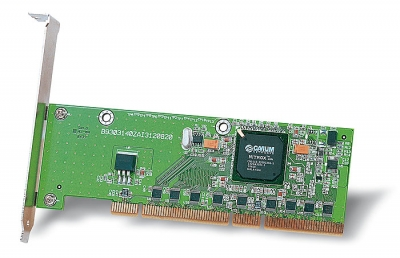
\includegraphics[scale=0.7]{pics/crypto-accelerator.eps}
\end{center}

\subsection{HTTP overload}
Ways to mitigate HTTP overload:

\begin{itemize}
	\item DNS round-robin to many web servers
	\item load balancing
	\item web cache / accelerators
	\item content delivery networks
\end{itemize}

These solutions depend on the location within the network and the scale of
the environment.

\subsection{Load Balancing}
\begin{center}
	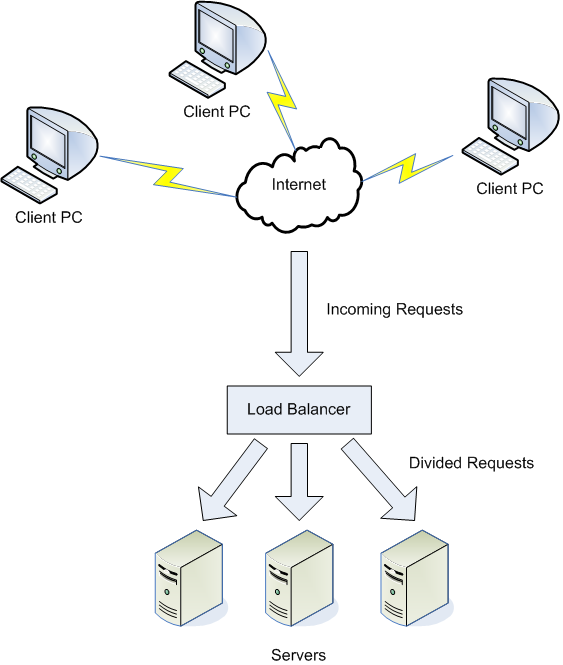
\includegraphics[scale=0.55]{pics/Lb101.eps}
\end{center}

\subsection{Load Balancing: Inbound}
\begin{center}
	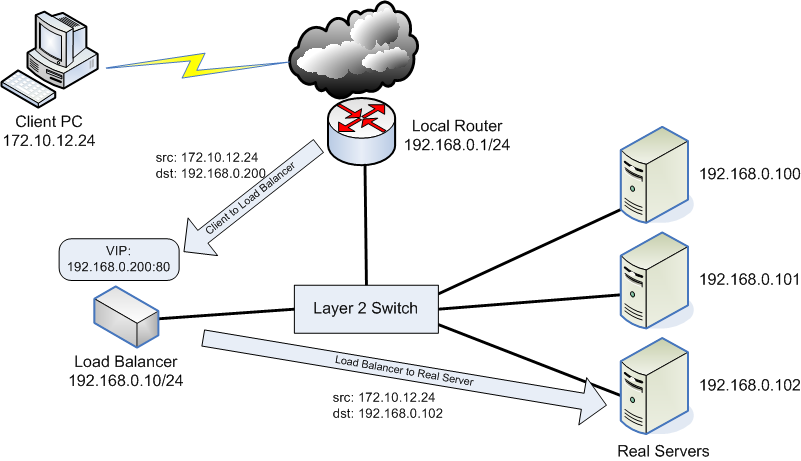
\includegraphics[scale=0.7]{pics/One-armed-inbound.eps}
\end{center}

\subsection{Load Balancing: Outbound}
\begin{center}
	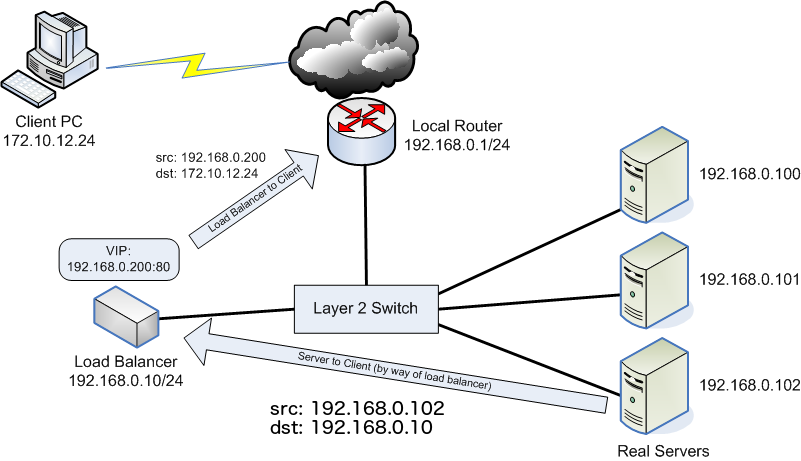
\includegraphics[scale=0.7]{pics/One-armed-outbound.eps}
\end{center}

\subsection{Load Balancing: Direct Server Return}
\begin{center}
	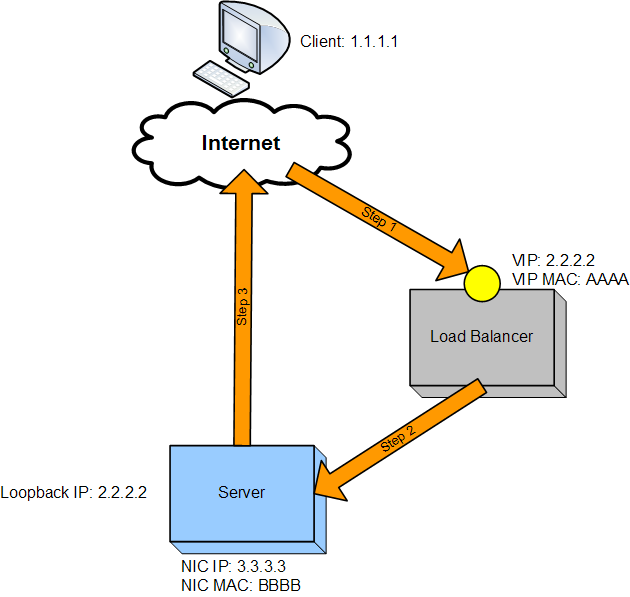
\includegraphics[scale=0.6]{pics/DSR.eps}
\end{center}

\subsection{Content Delivery Networks}
\begin{center}
	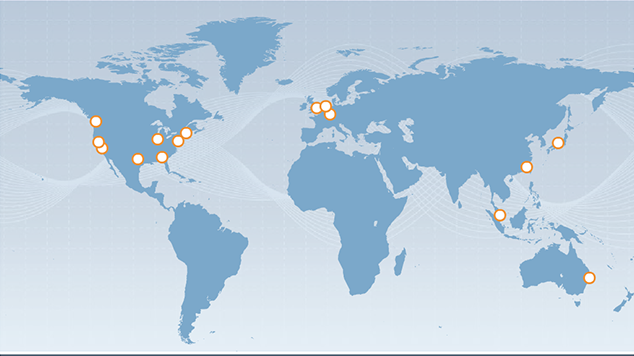
\includegraphics[scale=0.9]{pics/cdn.eps}
\end{center}

\subsection{Content Delivery Networks}
\begin{itemize}
	\item cache content in strategic locations
	\item determine location to serve from via geomapping of IP
		addresses (beware IPv6 aggregation!)
	\item often uses a separate domain to distinguish small
		objects/large objects or dynamic content/static content
	\item either out-sourced or in-house (if your organization is a
		Tier-1 or Tier-2 peering partner)
	\item request routing happens via Global Server Load Balancing,
		DNS-based request routing, anycasting etc.
	\item provides vast amounts of interesting data about your clients
		(see \verb+http://www.akamai.com/stateoftheinternet/+)
\end{itemize}

%\subsection{In-class exercise}
%\vspace{1in}
%\verb+http://www.cs.stevens.edu/~jschauma/615/http-exercise.html+


%%\subsection{The Apache webserver}
%%\begin{itemize}
%%	\item usually runs the {\em httpd} program as a d\ae mon
%%	\item usually runs as a dedicated user such as {\em nobody} or {\em www}
%%	\item can bind to specific IP-address/port pairs
%%	\item supports so-called {\em virtual hosts}
%%	\item supports a large number of {\em modules}, either specified at
%%		compile time or dynamically loaded modules.  Examples:
%%		\begin{itemize}
%%			\item {\em mod\_access} -- access control based on client
%%				hostname, IP address etc.
%%			\item {\em mod\_auth} -- user authentication
%%			\item {\em mod\_cgi} -- execution of CGIs
%%			\item {\em mod\_rewrite} --     rule-based rewriting engine to
%%				rewrite requested URLs on the fly
%%			\item {\em mod\_suexec} -- execution of CGIs as specified
%%				users/groups
%%		\end{itemize}
%%\end{itemize}
%%
%%\subsection{Apache Virtual Hosts}
%%{\em Virtual Hosts} allows you to run more than one web site on a single
%%machine.
%%\\
%%
%%\begin{itemize}
%%	\item {\em Virtual Hosts} can be
%%		\begin{itemize}
%%			\item IP-based
%%			\item port-based
%%			\item name-based
%%		\end{itemize}
%%	\item name-based {\em Virtual Hosts} do {\bf not} work with SSL
%%\end{itemize}
%%
%%
%%\subsection{Dynamic Content with CGI under Apache}
%%\begin{itemize}
%%	\item set {\em ScriptAlias} for a global directory
%%	\item use {\em AddHandler} / {\em SetHandler} to designate files or
%%		subdirectories as CGIs
%%	\item CGIs must produce a proper MIME-header
%%	\item things can go wrong:
%%		\begin{itemize}
%%			\item {\bf Internal Server Error} -- check logs.  Most likely
%%				cause of error: wrong permissions or missing MIME-header
%%			\item {\bf Forbidden} -- wrong permissions on file or directory
%%			\item you get source code of your CGI program or a {\bf POST Method
%%				Not Allowed} message -- Apache was not configured to allow
%%				execution of CGIs
%%		\end{itemize}
%%	\item use {\em mod\_suexec} to allow execution of CGIs as another user
%%		(for example, to access resources that {\em www} does not have access
%%		to)
%%\end{itemize}

%\newpage
%\vspace*{\fill}
%\begin{center}
%	\Hugesize
%		SSH\\ [1em]
%	\hspace*{5mm}
%	\blueline\\
%	\hspace*{5mm}\\
%		secure encrypted terminal sessions
%\end{center}
%\vspace*{\fill}
%
%\subsection{SSH}
%\vspace{.5in}
%\begin{center}
%	\Huge
%	``secure'' replacement for \verb+telnet+, \verb+rlogin+, \verb+rsh+
%\end{center}
%\Normalsize
%
%\subsection{SSH}
%Components:
%\begin{itemize}
%	\item \verb+sshd(8)+
%	\item \verb+ssh(1)+
%\end{itemize}
%
%\subsection{SSH}
%Components:
%\begin{itemize}
%	\item \verb+sshd(8)+
%	\item \verb+ssh(1)+
%	\item \verb+scp(1)+
%	\item \verb+sftp(1)+
%	\item \verb+ssh-agent(1)+
%	\item \verb+ssh-keygen(1)+
%\end{itemize}
%
%\subsection{SSH}
%Authentication done in primarily two modes:
%\begin{itemize}
%	\item password authentication
%	\item public-key authentication
%\end{itemize}
%
%\subsection{SSH}
%Authentication done in primarily two modes:
%\begin{itemize}
%	\item password authentication
%	\item public-key authentication
%\end{itemize}
%\vspace{.2in}
%Communication {\em always} envolves public-key encryption.
%
%\subsection{SSH}
%Authentication done in primarily two modes:
%\begin{itemize}
%	\item password authentication
%	\item public-key authentication
%\end{itemize}
%\vspace{.2in}
%Communication {\em always} envolves public-key encryption.
%\\
%
%Except when it doesn't (\verb+cipher:none+).
%
%\subsection{SSH}
%SSH {\em hostkeys}
%\begin{itemize}
%	\item each host has (at least) one private key
%	\item upon connection, it is verified against a public key
%	\item discrepancies are reported (and should be investigated!)
%	\item server and client perform a challenge-response handshake involving a
%		random number (which becomes the session key) in SSHv1 or via
%		Diffie-Hellman key agreement in SSHv2
%\end{itemize}
%
%\subsection{SSH}
%SSH {\em userkeys}
%\begin{itemize}
%	\item used during {\em public-key authentication}
%	\item the user has a {\em private} key
%	\item the remote host has the corresponding {\em public} key
%	\item the private key may be passphrase-protected
%	\item the passphrase used and the private key itself never leave the
%	      local host
%\end{itemize}
%
%\subsection{SSH}
%SSH {\em agents}:
%\begin{itemize}
%	\item allow the user to add multiple keys once, then no longer need to
%		provide the passphrases
%	\item agents can be {\em forwarded}
%	\item communication happens through a unix-domain socket
%\end{itemize}
%
%\subsection{SSH configuration}
%\vspace{.5in}
%\begin{center}
%	\Huge
%	\verb+sshd_config(5)+
%	\\
%	\verb+ssh_config(5)+
%\end{center}
%\Normalsize
%
\subsection{Reading}
HTTP etc.:
\begin{itemize}
	\item RFC 2616, 2818, 3875
	\item \verb+http://httpd.apache.org/docs/+
	\item \verb+http://www.w3.org/Protocols/+
	\item REST: \verb+http://is.gd/leSvGa+
	\item CDNs: \verb+http://is.gd/R5DoxA+
		\begin{itemize}
			\item \verb+http://www.edgecast.com/+
			\item \verb+https://aws.amazon.com/cloudfront/+
			\item \verb+http://www.akamai.com/+
			\item \verb+http://www.limelight.com/+
			\item ...
		\end{itemize}
	\item \verb+http://developer.yahoo.com/performance/rules.html+
\end{itemize}

\subsection{Reading}
SNMP:
\begin{itemize}
	\item \verb+http://is.gd/1LwOSD+
	\item RFCs 1157, 3411, 3418 and others
	\item \verb+snmpcmd(1)+
\end{itemize}
%
%\subsection{Reading}
%SSH:
%\begin{itemize}
%	\item \verb+ssh(1)+
%	\item \verb+ssh_config(5)+
%	\item \verb+sshd_config(5)+
%	\item \verb+sshd(8)+
%	\item RFC4255 -- SSHFP in DNS
%\end{itemize}
%
\end{document}
